\begin{center}
  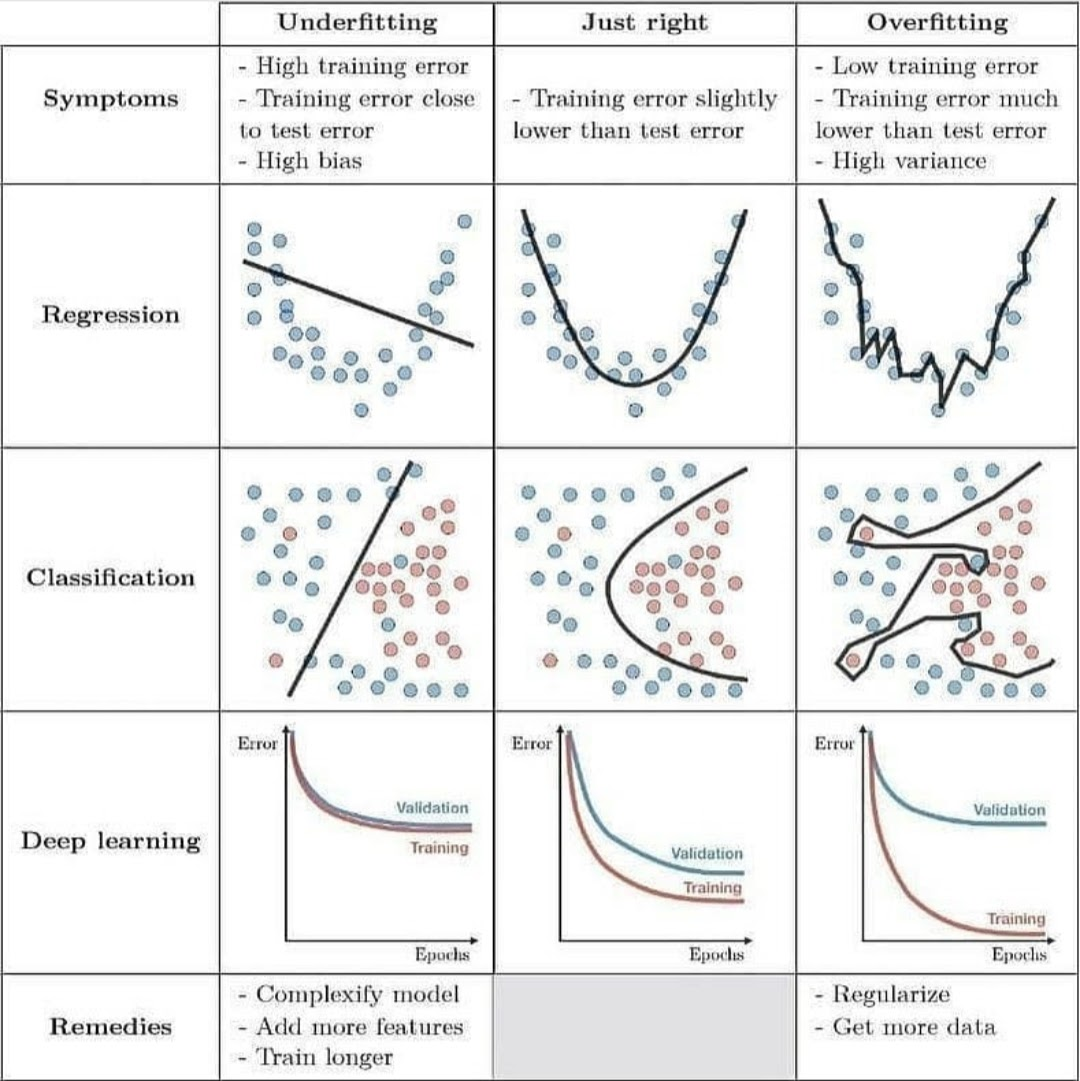
\includegraphics[width=0.8\textwidth]{overunderfitting.jpg}
\end{center}

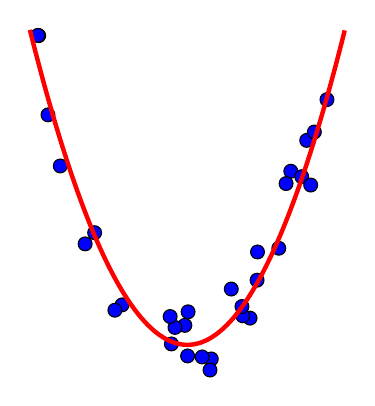
\begin{tikzpicture}[]
  \foreach \i in {0,...,30}{
    \pgfmathsetmacro{\x}{(rand)*2}
    \pgfmathsetmacro{\y}{(\x)^2 + (rand)/2}
    \node [circle,draw=black,fill=blue,minimum size=5pt,inner sep=0] (\i) at (\x,\y) {};
  }
  \draw[red,ultra thick,samples=100] plot[domain=-2.0:2.0] (\x,{(\x)^2});
\end{tikzpicture}


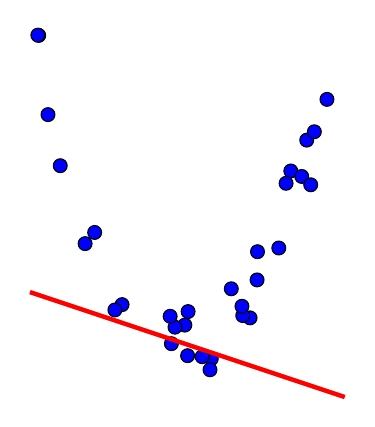
\begin{tikzpicture}[]
  \foreach \i in {0,...,30}{
    \pgfmathsetmacro{\x}{(rand)*2}
    \pgfmathsetmacro{\y}{(\x)^2 + (rand)/2}
    \node [circle,draw=black,fill=blue,minimum size=5pt,inner sep=0] (\i) at (\x,\y) {};
  }
  \draw[red,ultra thick,samples=100] plot[domain=-2.0:2.0] (\x,{-(\x/3)});
\end{tikzpicture}


\begin{tikzpicture}[]
  \foreach \i in {0,...,30}{
    \pgfmathsetmacro{\x}{(rand)*2}
    \pgfmathsetmacro{\y}{(\x)^2 + (rand)/2}
    \node [circle,draw=black,fill=blue,minimum size=5pt,inner sep=0] (n-\i) at (\x,\y) {};
    \pgfmathparse{\i - 1}
    \edef\last{n-\pgfmathresult}
    \draw[red,ultra thick] (\last) -- (n-\i);
  }
\end{tikzpicture}


%%% Local Variables:
%%% mode: latex
%%% TeX-master: "../figs"
%%% End:
